In this section the Alloy model is represented. The main and most important features and constraints of each TrackMe module has been modeled. More precisely the correctness of goal 4 has been checked for Dat4Help ("Provide data in an anonymous way, to protect user’s privacy"), for AutomatedSOS the goal 7 is checked ("Send an ambulance to user’s location whenever certain parameters are below the threshold") and furthermore for Track4Run the goal 10 is checked ("Allow spectators to watch in real time the position of every athlete in a specific run").
\bigbreak
\noindent
In order to see whether the model satisfy Data4Help's privacy constraint, the minimum number of group members has been dropped from 1000 to 3 so that the complexity of tests decreases without changing the model's logic. 

\subsection{Code}
\lstinputlisting[language=alloy]{Files/alloyCode.als}
\subsection{Results}
\begin{figure}[H]
\centering
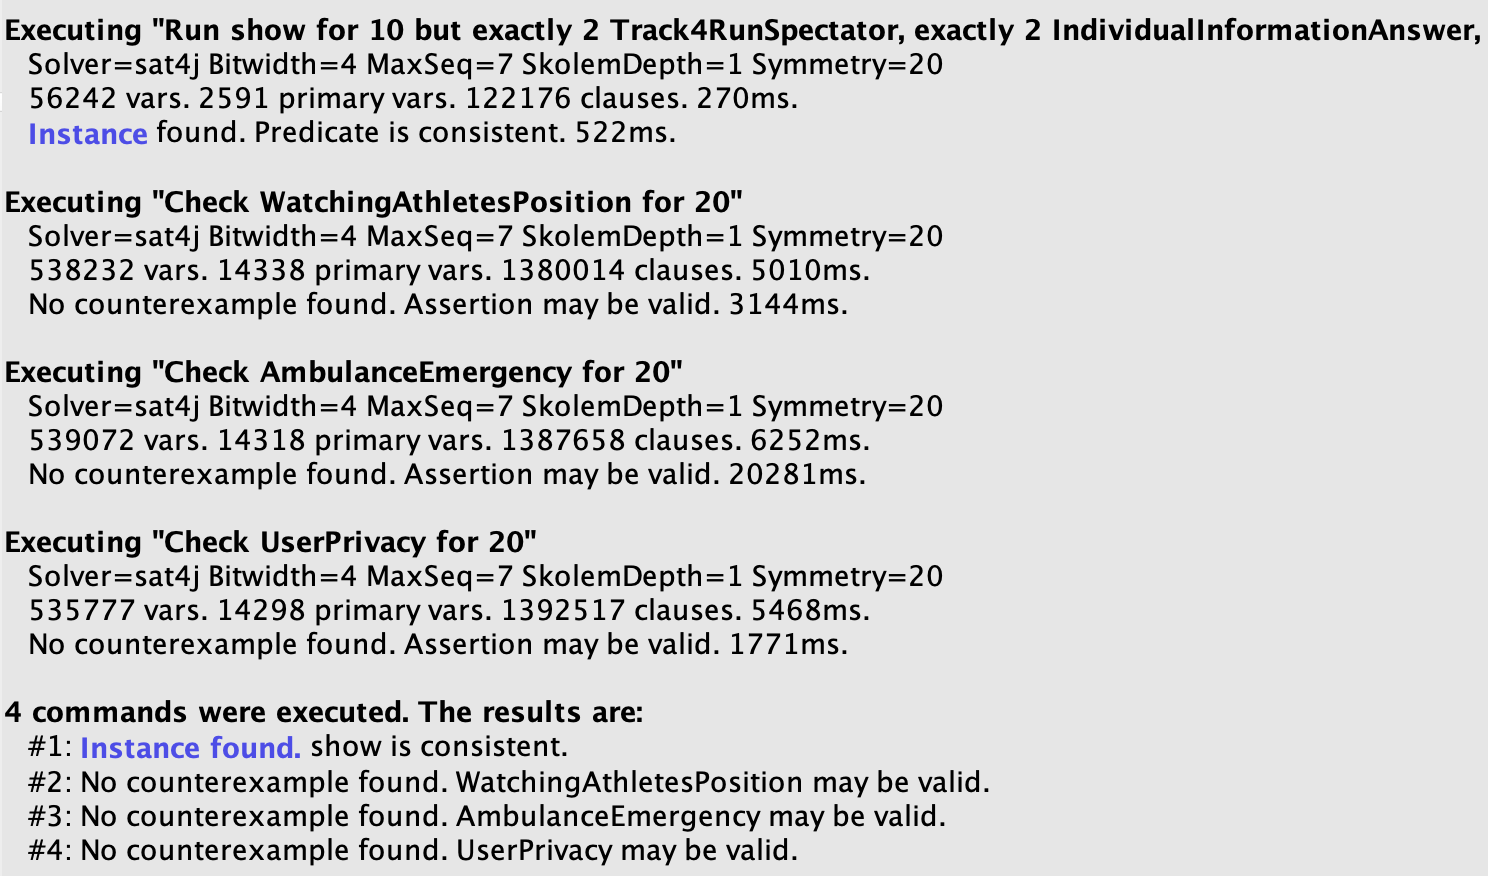
\includegraphics[scale=0.5]{Images/alloyResult.png}
\caption{Alloy Results}
\end{figure}
\clearpage
\subsection{Generated World}
\begin{figure}[H]
\centering
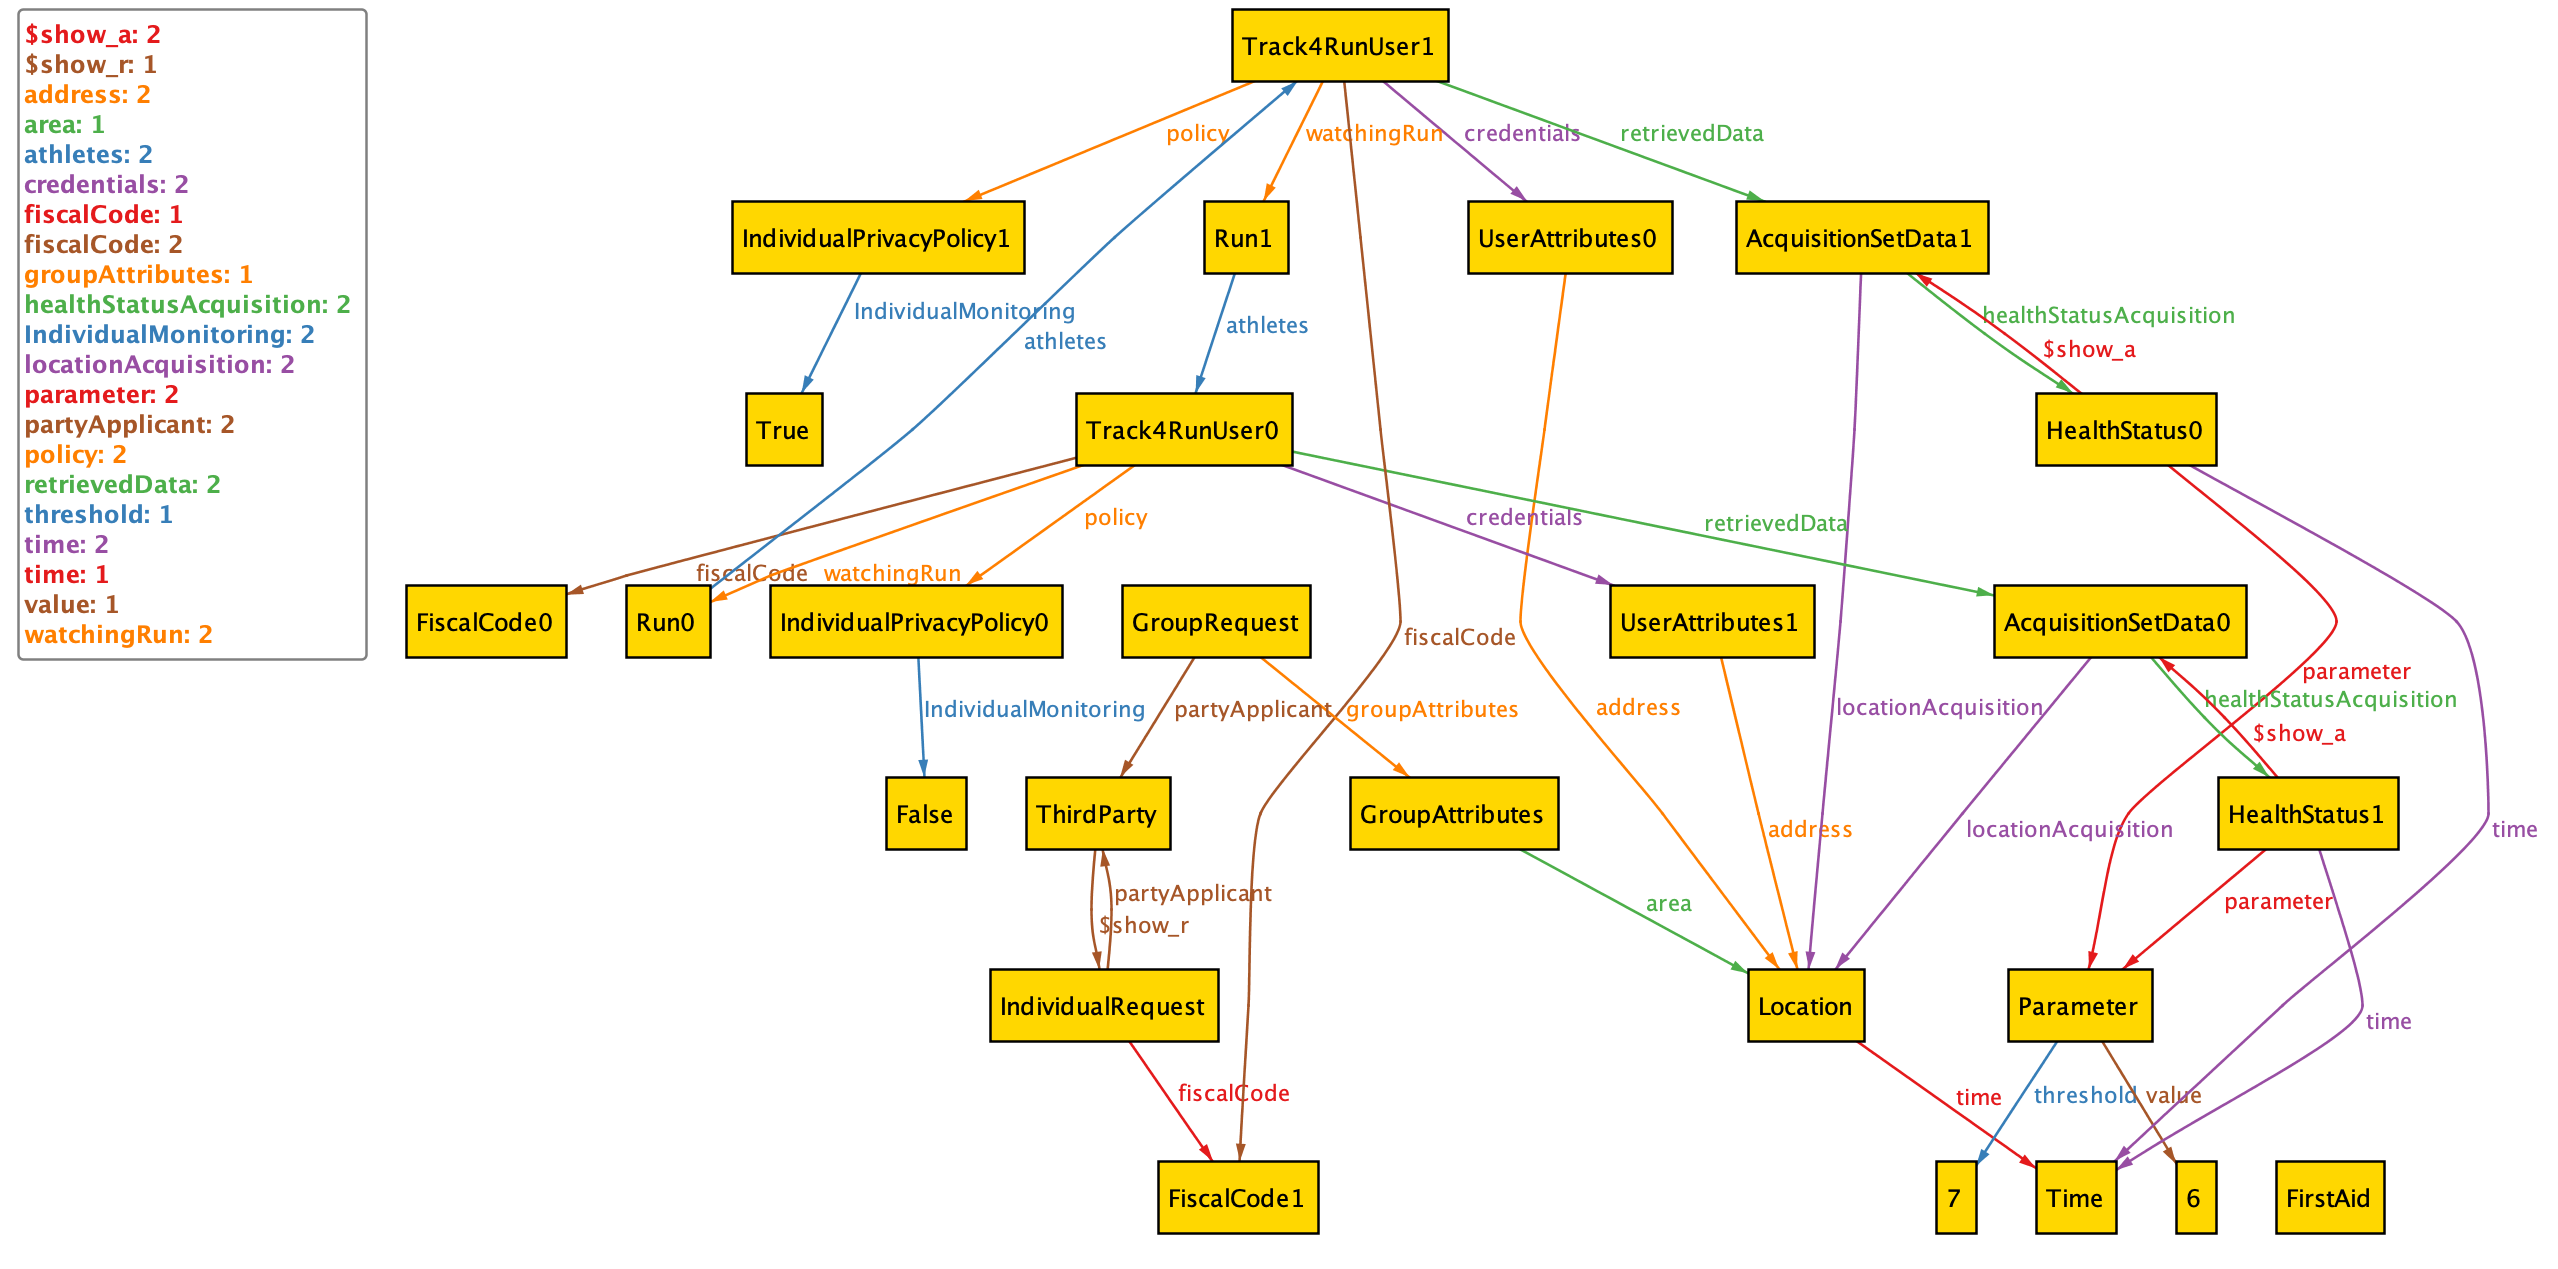
\includegraphics[scale=0.47, angle=-90,origin=c]{Images/alloyGeneratedWorld.png}
\caption{Sample of world generated by Alloy}
\end{figure}